\section{Durchführung}
\label{sec:Durchführung}

\begin{figure}
    \centering
    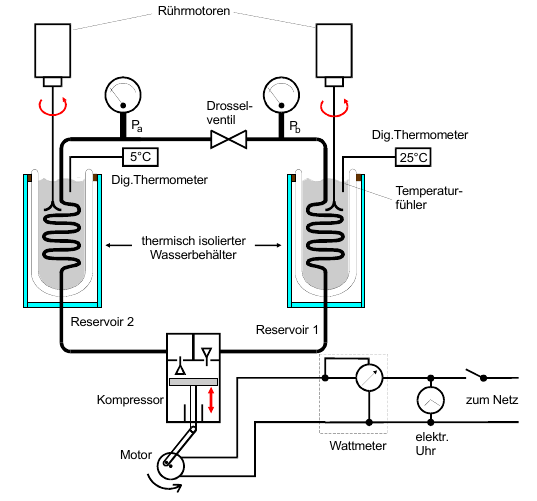
\includegraphics{WärmepumpeDurchführung.png}
    \caption{Versuchsaufbau}
    \label{fig:aufbau}
\end{figure}
Abbildung\ref{fig:aufbau} stellt den schematischen Versuchsaufbau einer
Wärmepumpe dar.\\
Zusätzlich zu den Grunbausteinen einer Wärmepumpe werden zwei digitale Thermometer 
und zwei Druckmessgeräte eingebaut um die Wärme in den Reservoiren und den Druck des 
Transportmediums zu bestimmen. Es müssen also die Reservoire mit einer genau abgemessenen
Wassermenge befüllt werden. Damit die Temperaturen während
der Messung genau sind, werden die Reservoire kontinuierlich
von Rührstäben vermischt. \\
Dann werden im Minutentakt die Temperaturen, die Drücke und
die Leistungsaufnahme des Kompressors gemessen. Abgebrochen 
werden die Messungen erst bei einer Temperatur von 50°C.

